\chapter{Технологический раздел}

\section{Язык программирования}
В качестве языка программирований выбран язык высокого уровня JavaScript.

\section{Примеры кода}

\begin{lstlisting}[caption={распределение Пуассона}]
function poissonPMF(x, lambda) {
    return Math.pow(Math.E, -lambda) * Math.pow(lambda, x) / factorial(x);
}

function poissonCDF(x, lambda) {
    let s = 0;
    for (let i = 0; i <= x; ++i) {
        s += poissonPMF(i, lambda);
    }

    return s;
}
\end{lstlisting}

\begin{lstlisting}[caption={Равномерное распределение}]
function uniformPMF(x, a, b) {
    if (x < a || x > b) return 0;

    return 1 / (b - a);
}

function uniformCDF(x, a, b) {
    if (x < a) return 0;
    if (x > b) return 1;
    
    return (x - a) / (b - a);
}
\end{lstlisting}

\section{Взаимодейсвтие с пользователем}

Взаимодейсвтие с пользователем осуществляется через html страницы, открытые в браузере.

\begin{figure}
  \centering
  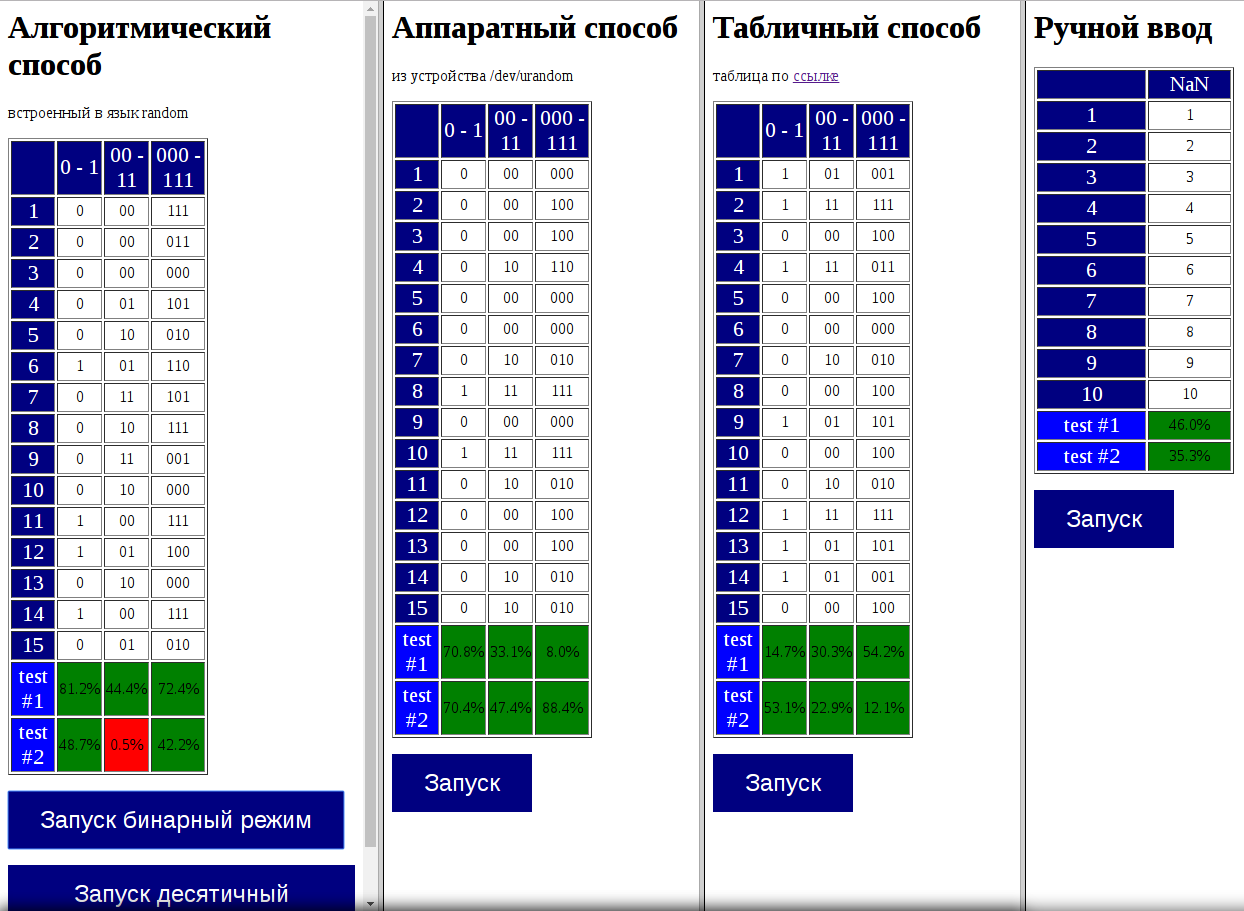
\includegraphics[scale=0.5]{screen1.png}
  \caption{Распределение Пуассона}
\end{figure}

\begin{figure}
  \centering
  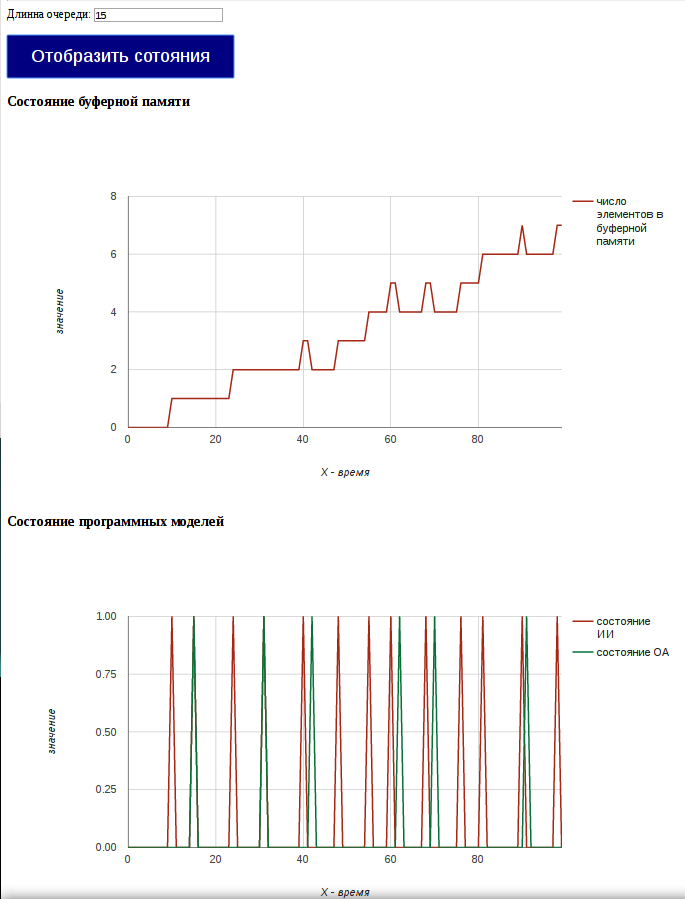
\includegraphics[scale=0.5]{screen2.png}
  \caption{Равномерное распределение}
\end{figure}
